\documentclass{article}

%-- packages --
\usepackage{xcolor}
\usepackage{tabularx}
\usepackage{array}
\usepackage{graphicx}
\usepackage[section]{placeins}
\usepackage{booktabs} 
\usepackage{multirow} 
\usepackage{caption} 
\usepackage{subcaption}

%-- setup --
\newtheorem{theorem}{Teorema}
\newcolumntype{C}{>{\centering\arraybackslash}X}
\graphicspath{ {graphs/} }

\title{Statistiche di ordine dinamiche}
\author{Tescaro Rocco}
\date{\today}

%-- document --
\begin{document}

\thispagestyle{plain}
\begin{center}
    \Large
    \textbf{Statistiche di ordine dinamiche}
    
    \vspace{0.2cm}
    \large
    Analisi comparativa implementazioni OS
    
    \vspace{0.4cm}
    \textbf{Tescaro Rocco}
    \vspace{0.2cm}
\end{center}

\section*{Introduzione}
\noindent Nel campo dell'analisi dei dati le statistiche di ordine dinamiche ricoprono un ruolo fondamentale per l'efficiente manipolazione di tali dati. Permettono di analizzare il comportamento, calcolare rapidamente la distribuzione relativa dei dati nelle strutture dati in cui questi sono memorizzati. Il concetto di statistiche di ordine è strettamente legato a quello di strutture dati aumentate, vale a dire strutture dati note, modificate memorizzando informazioni aggiuntive, al fine di implementare nuove funzionalità. In questo senso diverse strutture dati possono essere modificate in modo diverso per gestire efficientemente nuove operazioni come la funzione \textbf{os\_select(root, i)} o \textbf{os\_rank(root, key)}. \\

\noindent In questa relazione andremo ad analizzare la complessità temporale di diverse implementazioni, su diverse strutture dati, di statistiche di ordine dinamiche. In particolare confronteremo tre diverse implementazioni delle statistiche d'ordine dinamiche: la prima utilizzando una lista ordinata (\textbf{ordered\_list}), la seconda utilizzando un Albero Binario di Ricerca (ABR, \textbf{binary\_tree}) e la terza utilizzando una struttura dati aumentata consistente in un Albero Rosso-Nero (ARN) i cui nodi memorizzano la dimensione del sotto-albero di cui sono radice (\textbf{os\_tree}). \\

\noindent Come accennato le statistiche d'ordine su cui condurremo le nostre ricerche sono:
\begin{description}
    \item[os\_select(i)]: restituisce l'i-esimo elemento più piccolo memorizzato nella struttura dati che fornisce tale funzionalità. In particolare in un ARN aumentato per le statistiche d'ordine ha complessità $O(ln(n))$. Da notare come al contrario della funzione accennata prima non passeremo la radice di una struttura alla funzione ma questa essendo implementata direttamente dalle varie strutture dati userà la radice memorizzata da esse.
    \item[os\_rank(x)]: ritorna la posizione (rango) dell'elemento x relativamente ad un attraversamento ordinato della struttura dati analizzata. In un ARN aumentato ha complessità $O(ln(n))$. Allo stesso modo dell'os\_select non passeremo la radice ma solo l'elemento.
\end{description}

\section*{Strutture dati}

Come introdotto per la nostra analisi indagheremo il mantenimento e implementazione di statistiche d'ordine su diverse strutture dati, quali: lista ordinata, albero binario e albero rosso-nero aumentato. 

\subsection*{Lista ordinata}

\noindent La prima struttura dati che andremo ad analizzare è quella della lista ordinata. Una lista ordinata è un insieme di elementi, dove a ciascun elemento viene assegnata una posizione unica in base al valore di una chiave (generalmente con ordine crescente o decrescente). Questa proprietà permette in generale di inserire, ricercare e cancellare elementi rapidamente. \\

\noindent Ci sono diversi modi di implementare una lista ordinata, le proprietà citate infatti possono essere implementate su una qualsiasi struttura dati incidendo sulla complessità di alcuni metodi. Nel nostro caso useremo una lista doppiamente collegata con inserimento ordinato. Una lista doppiamente collegata è una struttura dati che consiste di un insieme di \textbf{nodi} in cui ogni nodo ha le seguenti attributi:

\begin{description}
    \item[value]: il valore, chiave su cui avverrà l'ordinamento. In quanto chiave deve supportare operatori di confronto.
    \item[prev]: puntatore al nodo predecessore
    \item[next]: puntatore al nodo successore
\end{description} 

\noindent Al contrario della lista collegata, la presenza dell'attributo \textbf{prev} (previous) permette un efficiente attraversamento della struttura in entrambe le direzioni. Per l'inserimento di un nodo la lista viene attraversata consequenzialmente a partire dal nodo iniziale fino al nodo con valore maggiore (in caso di ordinamento crescente) del nodo da inserire. Vengono quindi modificati gli attributi del nodo predecessore, del nodo stesso e del successore ai fini dell'inserimento. La cancellazione di un nodo avviene allo stesso modo ma ai fini dei nostri esperimenti non ne è necessaria l'implementazione. L'inserimento nel caso peggiore ha complessità  $O(n)$ con n pari al numero di elementi nella lista (il caso in cui l'elemento da inserire sia l'ultimo della lista). \\

\noindent Per quanto riguarda le statistiche d'ordine la selezione dell'i-esimo elemento può avvenire solo attraversando la lista dall'inizio (o dalla fine) con costo $O(i)$ questo comporta che nel caso peggiore la complessità sia sempre lineare $O(n)$. Anche per la funzione \textbf{os\_rank(root, key)} l'implementazione avviene con un attraversamento dal primo nodo sino a quello ricercato e dunque ha nel caso peggiore complessità $O(n)$ (nel caso il nodo non sia nella lista o l'ultimo della stessa).

\subsection*{Albero binario}
Un albero binario è una struttura dati gerarchica in cui ogni elemento è detto \textbf{nodo} ed ogni nodo ha al più due \textbf{nodi figli}, ai quali facciamo riferimento come figlio destro e figlio sinistro. In quanto albero è un grafo aciclico e il nodo \textit{iniziale} è detto \textbf{radice}. Come descritto ogni nodo ha al più due figli, un nodo senza figli è detto \textbf{foglia}. \\

\noindent Ogni nodo ha i seguenti attributi:
\begin{description}
    \item[value]: il valore, chiave su cui avverrà l'ordinamento. In quanto chiave deve supportare operatori di confronto.
    \item[parent]: puntatore al nodo predecessore
    \item[left]: puntatore al nodo figlio sinistro il cui valore è minore del valore del nodo stesso (albero binario crescente)
    \item[right]: puntatore al nodo figlio destro il cui valore è maggiore del valore del nodo stesso (albero binario crescente)
\end{description}

\noindent L'inserimento in un albero binario mira, oltre all'inserimento di un nuovo nodo stesso, a mantenere le proprietà dell'albero binario, assicurando che rimanga ben strutturato e organizzato (mantenendo le due proprietà degli alberi binari). L'inserimento avviene ricorsivamente iniziando dal nodo radice. Si confronta il valore del nuovo nodo da inserire con quello del nodo corrente. Se il valore del nuovo nodo è inferiore a quello del nodo corrente, ci spostiamo sul figlio sinistro del nodo corrente. Se il figlio sinistro è vuoto, si inserisce il nuovo nodo come figlio sinistro del nodo corrente. Se il figlio sinistro non è vuoto, si ripete ricorsivamente il processo di inserimento partendo dal figlio sinistro. Se invece il valore del nuovo nodo è maggiore di quello del nodo corrente, ci si sposta sul figlio destro del nodo corrente. Se il figlio destro è vuoto, inseriamo il nuovo nodo come figlio destro del nodo corrente. Se il figlio destro non è vuoto, si ripete ricorsivamente il processo di inserimento partendo dal figlio destro. La complessità nel caso medio è $O(ln(n))$ tuttavia se l'albero è sbilanciato, vale a dire se ad esempio l'inserimento è avvenuto con valori ordinati, la struttura non è dissimile da quella della lista doppiamente collegata e la complessità sarà $O(n)$.  \\

\noindent Per la complessità delle due funzioni di statistiche d'ordine la complessità nel caso peggiore, come in quello medio è pari alla complessità di un'\textit{inorder-walk} vale a dire lineare, $O(n)$.

\subsection*{Albero rosso-nero aumentato}
L'albero rosso e nero aumentato è una variante dell'albero di ricerca binario bilanciato o albero rosso-nero, una struttura dati aumentata, in questo caso, al fine di implementare efficientemente le statistiche di ordine dinamiche. In un albero rosso-nero a ogni nodo viene assegnato un colore: rosso o nero. L'albero viene mantenuto in modo bilanciato per garantire operazioni efficienti come l'inserimento, la cancellazione e la ricerca. \\

\noindent Ogni nodo ha quindi i seguenti attributi: 

\begin{description}
    \item[value]: il valore, chiave su cui avverrà l'ordinamento. In quanto chiave deve supportare operatori di confronto.
    \item[parent]: puntatore al nodo predecessore
    \item[left]: puntatore al nodo figlio sinistro il cui valore è minore del valore del nodo stesso (sempre ordinamento crescente)
    \item[right]: puntatore al nodo figlio destro il cui valore è maggiore del valore del nodo stesso (sempre ordinamento crescente)
    \item[color]: valore binario che indica il colore del nodo. Nel nostro caso implementato come valore booleano: \textbf{True} per il rosso, \textbf{False} per il nero
    \item[size]: dimensione, numero di elementi del sotto-albero con radice il nodo stesso
\end{description}

\noindent L'albero aumentato rosso e nero mantiene la sua struttura bilanciata attraverso l'uso di operazioni di rotazione e inversione dei colori, seguendo le proprietà dell'albero rosso e nero. Ulteriori modifiche vengono apportate durante l'inserimento, la cancellazione o altre operazioni per aggiornare le informazioni sulle dimensioni dei nodi, a seconda delle necessità. L'inserimento in un albero rosso-nero ha complessità logaritmica $O(lg(n))$ inoltre per il teorema: 
\begin{theorem}
Sia ${f}$ un campo che aumenta un ARN T di n nodi e supponiamo che il contenuto di ${f}$ per un nodo ${x}$ possa essere calcolato usando solo le informazioni nei nodi ${x}$, ${x.left}$ e ${x.right}$, inclusi ${x.left.f}$ e ${x.right.f}$. Quindi, possiamo mantenere i valori di ${f}$ in tutti i nodi di T durante l'inserimento e la cancellazione senza influenzare asintoticamente le prestazioni $O(lg(n))$ di queste operazioni.
\end{theorem}
anche l'inserimento per la versione aumentata ha complessità logaritmica $O(lg(n))$ (solo con costanti maggiori). \\

\noindent Per quanto riguarda le funzioni per le statistiche d'ordine dinamiche possono essere implementate così da avere sia nel caso peggiore che in quello medio complessità logaritmica $O(lg(n))$.

\section*{Analisi e Confronto}
\noindent Descritte le diverse strutture dati procediamo con la descrizione delle indagini che condurremo. In particolare verificheremo le complessità introdotte nella sezione precedente per le due funzioni. Cronometreremo il tempo di esecuzione per le diverse strutture dati su diversi \textit{dataset} di dimensioni che vanno da 10 elementi fino a 1000, con step da 10. \\

\noindent Il tempo verrà misurato con la libreria python \textbf{time} ma per una verifica più accurata conteremo anche il numero di nodi attraversati durante le singole esecuzioni. Le misurazioni temporali saranno in nanosecondi usando la funzione \textbf{perf\_counter\_ns()} che avendo accesso al process counter dovrebbe limitare i rallentamenti e quindi errori di misurazioni dovuti al sistema. Oltre a variare la dimensione dei dataset eseguiremo questi test per 1000 volte per ciascuna dimensione, per poi trarne la media e deviazione standard in modo da ammortizzare i risultati di casi sfavorevoli. \\

\noindent Ciascun dataset verrà generato con valori pseudocasuali usando la libreria \textbf{random}, cercando quindi di non occorrere in alberi binari non bilanciati o casistiche particolarmente svantaggiose. Ad ogni iterazione per il calcolo della media su una dimensione ciascuna delle strutture dati verrà rinizializzata e riempita con nuovi valori (questo farà aumentare il tempo di \textit{testing} ma ci assicurerà una maggiore accuratezza dei dati d'osservazione nei casi limite). I test saranno condotti sulla macchina descritta nell'appendice. \\

\noindent Ci aspettiamo che i risultati verifichino le complessità descritte nella sezione precedente, che ci sia una variazione sostanziale in risposta al crescere della dimensione del dataset. In particolare ci aspettiamo che gli alberi bilanciati rosso-neri aumentati presentino tempi migliori rispetto alle altre implementazioni. \\

\noindent Tra le varie problematiche che potremmo incontrare c'è l'aleatorietà nella generazione dei casi di test, che può determinare misure di prestazioni diverse per ogni esecuzione. Altre problematiche potrebbero sorgere dalle limitazioni dell'hardware e del sistema, L'ambiente hardware e di sistema può influenzare le misurazioni del tempo di esecuzione dati ad esempio processi in background, rallentamenti dati dallo scheduling o dal caching della memoria. Inoltre grandi dimensioni di input possono comportare limitazioni pratiche in termini di utilizzo della memoria o di tempo di esecuzione (python mette un limite al numero di ricorsioni dettata dalla limitatezza della dimensione dello stack e questo potrebbe influenzare le misurazioni per le ultime due strutture dati). \\

\noindent In generale data la finitezza delle dimensioni, operatori e singoli dataset su cui verranno eseguiti i test ci aspettiamo un margine di errore (minore nella seconda analisi che consiste nel conteggio dei nodi attraversati). 

\newpage

\section*{Dati sperimentali}

\noindent Dall'esecuzione del codice risultano i seguenti dati: \\

\begin{figure}[htbp]
    \caption{\textbf{os\_select}}
    \centering
    \begin{subfigure}[b]{0.45\textwidth}
        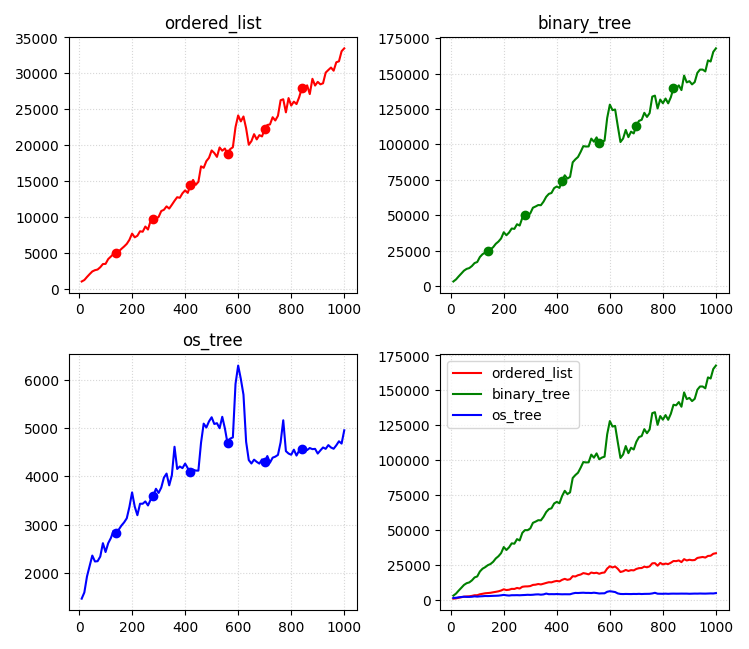
\includegraphics[width=\linewidth]{graphs1}
        \small
        \caption{grafico dei tempi}
    \end{subfigure}
    \hfill
    \begin{subfigure}[b]{0.45\textwidth}
        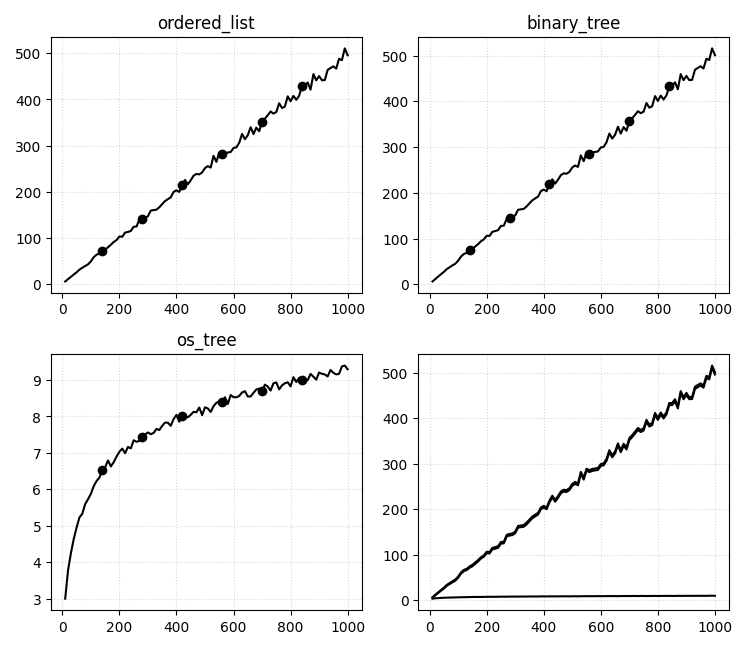
\includegraphics[width=\linewidth]{graphs2}
        \caption{grafico dei nodi esplorati}
    \end{subfigure}    
\end{figure} 

Da un'indagine preliminare notiamo che i grafici a) e b) riportano dati molto simili a meno della grandezza fisca dei dati ovviamente rispettano lo stesso andamento), molti \textit{spikes} sono comuni a tutti i grafici a) ma non non sono presenti nei grafici b), questo indica che probabilmente i problemi individuati relativamente all'hardware e il sistema operativo si sono dimostrati realistici, processi in background hanno determinato un allungamento dei tempi di esecuzione. Altri \textit{spikes} invece sono comuni sia ai grafici dei tempi che dei nodi esplorati, questo indica che ci sono stati più tentativi sfavorevoli, con ad esempio la ricerca di valori alti nelle diverse strutture dati. In generale comunque la complessità teorizzata sembra verificata sia in termini di tempi fisici che in numero di nodi esplorati. 

\begin{figure}[htbp]
    \caption{\textbf{os\_rank}}
    \centering
    \begin{subfigure}[b]{0.45\textwidth}
        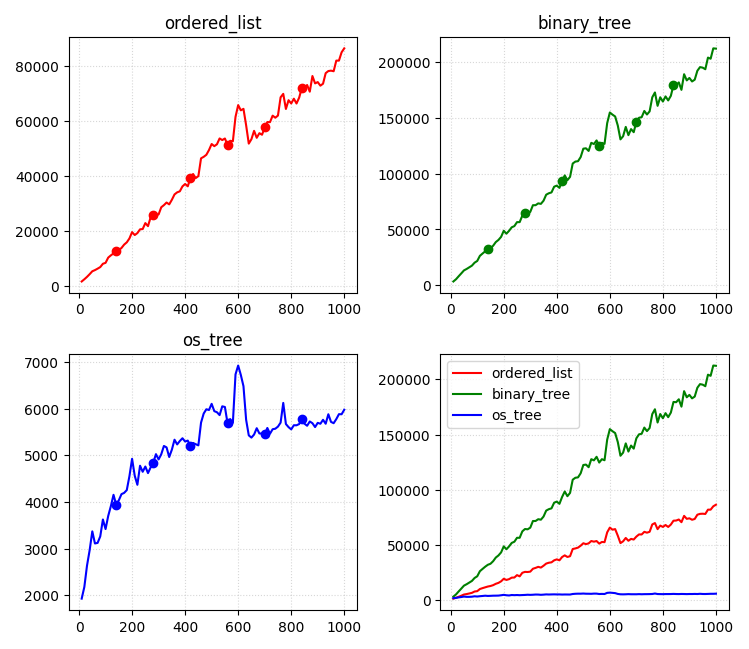
\includegraphics[width=\linewidth]{graphs3}
        \small
        \caption{grafico dei tempi}
    \end{subfigure}
    \hfill
    \begin{subfigure}[b]{0.45\textwidth}
        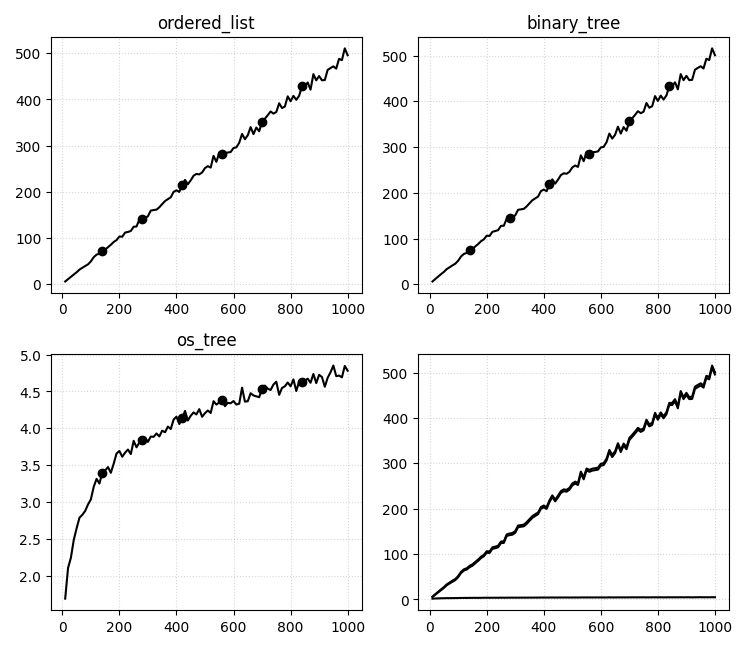
\includegraphics[width=\linewidth]{graphs4}
        \caption{grafico dei nodi esplorati}
    \end{subfigure}    
\end{figure}

\noindent A meno delle unità di grandezza l'andamento dei grafici dell'os\_select e dell'os\_rank corrispondono il che è promettente dato che le complessità attese, come premesso dalla sezione precedente, sono le stesse.\\

\noindent Avendo effetuato le nostre misurazioni su una mole notevole di dati (99 dimensioni diverse) riportiamo i risultati in tabella solo di 6 di queste, da 140 a 840 con step da 140 (che concidono anche con i punti dei grafici). 

\begin{figure}[h]
    \caption{Risultati cronometraggio statistiche di ordine dinamico: \textbf{ordered\_list}}
        \begin{tabularx}{\textwidth}{ccccccc}
            \toprule
            \multirow{2}{*}{dim.} & \multicolumn{3}{c}{\textbf{os\_select}} & \multicolumn{3}{c}{\textbf{os\_rank}} \\
            \cmidrule(lr){2-4} \cmidrule(lr){5-7}
            & time (ns) & exp. nodes & std & time (ns) & exp. nodes & std. \\
            \midrule
140 & 4984.40 & 70.93 & 2549.22 & 12457.20 & 70.93 & 7116.52 \\
280 & 9718.40 & 141.77 & 5567.09 & 25718.20 & 141.77 & 15740.34 \\
420 & 14442.20 & 214.69 & 10762.10 & 39150.60 & 214.69 & 24326.81 \\
560 & 18778.20 & 281.31 & 10184.26 & 51274.20 & 281.31 & 28499.21 \\
700 & 22250.20 & 351.47 & 12708.17 & 57635.60 & 351.47 & 34125.87 \\
840 & 27917.80 & 428.76 & 15546.61 & 72033.20 & 428.76 & 41777.05 \\
140 & 24926.20 & 73.93 & 13435.27 & 32124.20 & 73.93 & 18041.71 \\
            \bottomrule
        \end{tabularx}
\end{figure}

\begin{figure}[h]
    \caption{Risultati cronometraggio statistiche di ordine dinamico: \textbf{binary\_tree}}
        \begin{tabularx}{\textwidth}{ccccccc}
            \toprule
            \multirow{2}{*}{dim.} & \multicolumn{3}{c}{\textbf{os\_select}} & \multicolumn{3}{c}{\textbf{os\_rank}} \\
            \cmidrule(lr){2-4} \cmidrule(lr){5-7}
            & time (ns) & exp. nodes & std & time (ns) & exp. nodes & std. \\
            \midrule
140 & 24926.20 & 73.93 & 13435.27 & 32124.20 & 73.93 & 18041.71 \\
280 & 50021.60 & 145.36 & 30147.68 & 64506.60 & 145.36 & 39044.02 \\
420 & 74398.00 & 218.58 & 42576.63 & 93509.80 & 218.58 & 54209.09 \\
560 & 100683.40 & 285.62 & 55102.07 & 124638.00 & 285.62 & 69579.83 \\
700 & 113223.60 & 355.87 & 65536.15 & 146563.60 & 355.87 & 89569.79 \\
840 & 139693.80 & 433.30 & 78913.29 & 179489.80 & 433.30 & 102215.36 \\
            \bottomrule
        \end{tabularx}
\end{figure}

\begin{figure}[h]
     \caption{Risultati cronometraggio statistiche di ordine dinamico: \textbf{os\_tree}}
        \begin{tabularx}{\textwidth}{ccccccc}
            \toprule
            \multirow{2}{*}{dim.} & \multicolumn{3}{c}{\textbf{os\_select}} & \multicolumn{3}{c}{\textbf{os\_rank}} \\
            \cmidrule(lr){2-4} \cmidrule(lr){5-7}
            & time (ns) & exp. nodes & std & time (ns) & exp. nodes & std. \\
            \midrule
140 & 2825.80 & 6.54 & 721.83 & 3945.00 & 3.40 & 997.23 \\
280 & 3601.80 & 7.43 & 986.07 & 4846.40 & 3.84 & 1288.32 \\
420 & 4093.60 & 8.01 & 865.22 & 5193.80 & 4.13 & 1031.65 \\
560 & 4682.20 & 8.41 & 1061.48 & 5686.80 & 4.38 & 1262.86 \\
700 & 4307.20 & 8.70 & 935.22 & 5457.60 & 4.54 & 1139.19 \\
840 & 4569.80 & 9.01 & 1033.47 & 5780.00 & 4.63 & 1634.14 \\
            \bottomrule
        \end{tabularx}
\end{figure}

\section*{Conclusioni e Discussione dati}

Come già osservato i grafici rispettano perlopiù l'andamento predetto dal comportamento limite delle complessità. La lista ordinata e l'albero binario infatti hanno un andamento lineare mentre l'os\_tree logaritmico. \\

\noindent Osservando più accuratamente però i dati relativi ai tempi di computazione per l'albero binario possiamo notare come questi siano più lunghi dei corrispettivi della lista ordinata. Ciò è probabilmente da attribuire al costo delle singole operazioni dei due algoritmi che nella seconda struttura dati sono probabilmente più costose, in particolare l'allocazione di memoria nello \textbf{stack} per le varie chiamate ricorsive può essere la causa di questa discrepanza. \\

\noindent Possiamo poi notare che la deviazione standard sia nel caso della lista ordinata (Figura 3) e dell'albero binario (Figura 4) è sempre circa la metà dei tempi calcolati (per la dimensione 560 della lista ordinata lo scarto quadratico medio relativo è del 54.23\%), questo implica che nei vari cronometraggi di ogni dimensione ci sono stati diversi risultati molto distanti fra loro, più precisamente ad esempio, il 68\% dei cronometraggi della lista ordinata con dimensione 560 ricade fra [8593.94, 28962.46] ([tempo - std, tempo + std]). Per quanto riguarda invece la deviazione standard per l'albero bilanciato aumentato (Figura 5) è di circa un quarto (per la dimensione 560 lo scarto quadratico medio relativo è del 22.67\%). Ciò è sempre da attribuire alla complessità per le rispettive strutture dati, la complessità minore nell'albero rosso-nero comporta una maggiore consistenza nei tempi complessivi di esecuzione dei due algoritmi. 

\vfill
\noindent\makebox[\linewidth]{\rule{\textwidth}{0.01pt}}
\footnotesize
appendice:

specifiche hardware e software
\centering
\begin{tabularx}{\textwidth}{|>{\hsize=2.\hsize}C|*{4}{>{\hsize=0.5\hsize}C|}}
    \hline
     \textbf{Processor} & \textbf{RAM} & \textbf{System type} & \textbf{OS edition} & \textbf{OS version} \\
     \hline
     AMD Ryzen 7 5700U with Radeon Graphics 1.80 GHz & 16.0 GB & 64-bit & Windows 11 Home & 22H2 \\
     \hline
\end{tabularx}

\end{document}
